\section{System Model}
\label{sec:system}

We consider a LEO satellite-enabled grant-free random access system
as illustrated in Fig.~\ref{fig:system-multiframe}, where AFDM is adopted
to mitigate the doubly dispersive effect \cite{huang2026} inherent in
terrestrial-satellite links (TSLs). The system comprises $K$
single-antenna terrestrial devices that communicate with a LEO satellite
equipped with a uniform planar array (UPA) consisting of $M=M_yM_z$
antennas. During each transmission block, active devices share the same
time-frequency resources to transmit their pilots to the satellite.
Additionally, we assume that these terrestrial devices operate without
GNSS assistance and do not pre-compensate for delay and Doppler shifts
\cite{shen2025}.

\begin{figure}[!t]
\centering
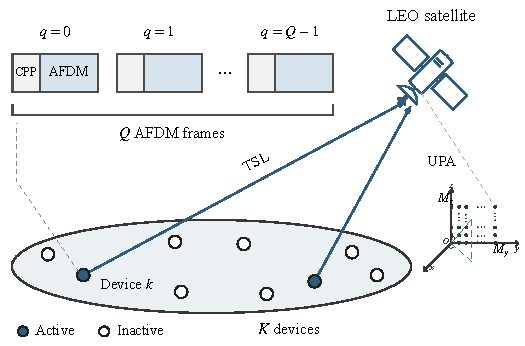
\includegraphics[width=\linewidth]{system_multiframe.pdf}
\caption{LEO satellite grant-free access with multi-frame AFDM pilot
transmission. The insets show the frame structure of active device $k$
and the satellite UPA. Device activity is fixed over the $Q$ frames.
Satellite, footprint, and array artwork
is adapted from \cite{shen2025}.}
\label{fig:system-multiframe}
\end{figure}

\subsection{Terrestrial-Satellite Link Model}

The TSLs experience fast variations due to the high mobility of the LEO
satellite. Hence, this time variation and multipath propagation require a
doubly dispersive channel model for accurate TSL characterization
\cite{shen2025}. For stationary terrestrial devices, the Doppler shift
$\nu_k$ is assumed to be common to all propagation paths within the same
TSL, since the long satellite-to-ground distance leads to only a small
angular spread across multipath components \cite{huang2026}.
The angles of arrival of these paths are approximately identical,
so that they
share the same array response vector $\mathbf a_k$ \cite{li2023}.
We assume that the channel in the delay-Doppler domain remains
approximately constant over the $Q$ frames of a transmission block
\cite{shen2025}. Then, taking the start of the block as $t_{\rm c}=0$,
the channel impulse response from the $k$th device to the satellite
after common-delay compensation by $\tau_{\rm c}$ can be represented as

\begin{equation}
 \mathbf h_k(t_{\rm c},\tau)
 =\mathbf a_k\sum_{\ell=1}^{L_k}g_{k\ell}
 e^{\mathrm j2\pi\nu_k t_{\rm c}}\delta(\tau-\tau_{k\ell}),
 \label{eq:physical-channel}
\end{equation}
where $k=1,\ldots,K$, and $L_k$ is the number of physical paths.
Here, $\tau_{k\ell}=\widetilde\tau_{k\ell}-\tau_{\rm c}$ represents the
differential delay for the $\ell$th path from the $k$th device to the
satellite, where $\widetilde\tau_{k\ell}$ and $\tau_{\rm c}$ denote the
propagation delay and common delay, respectively.
The common delay corresponds to the propagation time between the satellite
and the closest point on Earth within the beam footprint. Additionally,
$g_{k\ell}$ is the path gain of the $\ell$th path, $\delta(\cdot)$ is the
Dirac delta function, and $\mathrm j^2=-1$.

Then, the array response vector $\mathbf a_k$ can be expressed as
\begin{equation}
 [\mathbf a_k]_{n_z+M_zn_y}
 =e^{\mathrm j2\pi(d_yn_y\mu_{y,k}+d_zn_z\mu_{z,k})/\lambda},
 \label{eq:upa}
\end{equation}
where $n_z=0,\ldots,M_z-1$, $n_y=0,\ldots,M_y-1$,
$\lambda$ is the wavelength, and $d_y$ and $d_z$ are the spacings between
adjacent antennas along the $y$- and $z$-axes, respectively. The
directional cosines along these two axes are denoted by $\mu_{y,k}$ and
$\mu_{z,k}$, respectively.

\subsection{Transmission Scheme}
\label{sec:transmission-scheme}

The multi-frame AFDM transmission scheme is proposed to handle the large
differential delay and Doppler shift. In this scheme, each active device
transmits pilots over $Q$ consecutive frames within one transmission
block. While AFDM modulation and demodulation are performed separately
for each frame, the receiver jointly processes the resulting observations.
Specifically, in the $q$th AFDM frame, $q=0,\ldots,Q-1$, the $k$th
device transmits the known pilot vector $\mathbf p_{qk}\in\mathbb C^N$,
where $N$ is the number of chirp subcarriers shared by the devices.

We construct the pilot matrices as
$\mathbf P_k=[\mathbf p_{0k},\ldots,\mathbf p_{Q-1,k}]^{\mathsf T}$
and $\mathbf P=[\mathbf P_1,\ldots,\mathbf P_K]\in\mathbb C^{Q\times KN}$,
where $(\cdot)^{\mathsf T}$ denotes transpose.
We impose the condition that
$\mathbf P\mathbf P^{\mathsf H}=KE_p\I_Q$, where
$\|\mathbf p_{qk}\|^2=E_p$ for all $k$ and $q$
\cite{cai2026}.

Through the inverse discrete affine Fourier transform (IDAFT)
\cite{ding2026}, $\mathbf p_{qk}$ is mapped to the time-domain signal
given by

\begin{equation}
 s_{qk}[t]=\frac{1}{\sqrt N}\sum_{n=0}^{N-1}
 [\mathbf p_{qk}]_ne^{\mathrm j2\pi(c_1t^2+c_2n^2+nt/N)},
 \label{eq:afdm-time-signal}
\end{equation}
where $t=0,\ldots,N-1$, and $c_1$ and $c_2$ are AFDM modulation
parameters.
The corresponding discrete affine Fourier transform (DAFT) matrix is
\begin{equation}
 \begin{gathered}
 \mathbf F_{\rm A}
 =\left[\frac{1}{\sqrt N}e^{-\mathrm j2\pi(c_2r^2+rt/N+c_1t^2)}
 \right]_{r,t=0}^{N-1}
 \end{gathered}.
 \label{eq:daft}
\end{equation}

Assume that the chirp-periodic prefix (CPP) duration is greater than
or equal to the maximum differential delay, i.e.,
$N_{\rm CPP}T_s\geq\max_{k,\ell}\tau_{k\ell}$.
Here $T_s=1/(N\Delta f)$ is the sampling interval, with $\Delta f$
denoting the subcarrier spacing, and
$T_{\rm frame}=(N+N_{\rm CPP})T_s$ is the duration of an AFDM frame
with CPP.

Next, we use a continuous-time AFDM waveform
\cite{bemani2023thesis} with a chirp-periodic prefix extension
\cite{bemani2022} to model fractional delays. The basis function for
chirp subcarrier $n$ at time $\xi T_s$ is given by
\begin{equation}
 \varphi_n(\xi)=\frac{1}{\sqrt N}
 e^{\mathrm j2\pi[c_2n^2+c_1\xi^2+nw_\xi/N-\zeta_n(w_\xi)w_\xi]},
 \label{eq:continuous-waveform}
\end{equation}
where $w_\xi=\langle\xi\rangle_N$,
$\langle x\rangle_N=x-N\lfloor x/N\rfloor$,
$\zeta_n(w)=\lfloor2c_1w+n/N\rfloor$, and $2Nc_1\in\mathbb N_+$.

After CPP removal and DAFT demodulation, the effective channel from the
$k$th device to the satellite in frame $0$ can be expressed as
\begin{equation}
 \mathbf H_k=\mathbf a_k^{\mathsf T}\otimes
 \left[\sum_{\ell=1}^{L_k}g_{k\ell}
 \mathbf G(\tau_{k\ell}/T_s,\nu_k;N_{\rm CPP})\right]^{\mathsf T},
 \label{eq:channel}
\end{equation}
where $\mathbf H_k\in\mathbb C^{N\times MN}$ and $\otimes$ denotes
the Kronecker product. Here, $\mathbf G(d,\nu;g)$ represents the response
of a unit-gain path with delay $dT_s$ and Doppler shift $\nu$, given by

\begin{equation}
 \mathbf G(d,\nu;g)=\mathbf F_{\rm A}
 \left[e^{\mathrm j2\pi\nu T_s(g+t)}\varphi_n(t-d)\right]_{t,n=0}^{N-1}.
 \label{eq:path-operator-system}
\end{equation}
Here $t_{\rm c}=(g+t)T_s$ for $t=0,\ldots,N-1$ after removing
the CPP, and $g=N_{\rm CPP}$ for frame $0$.

In frame $q$, the useful samples start at time
$N_{\rm CPP}T_s+qT_{\rm frame}$. Since all paths of device $k$ share
the Doppler shift $\nu_k$, the effective channel in frame $q$ can be
expressed as
\begin{equation}
 \mathbf H_k^{(q)}=e^{\mathrm jq\beta_k}\mathbf H_k,
 \label{eq:twc-frame-channel}
\end{equation}
where $\beta_k\equiv2\pi\nu_kT_{\rm frame}\pmod{2\pi}$
and $\beta_k\in[-\pi,\pi)$.
Under the quasi-static assumption, $\mathbf H_k$ remains approximately
constant over the $Q$ frames. For example, consider a circular orbit and
a ground device in the orbital plane with an initial elevation angle of
$50^\circ$. The simulation parameters with $Q=16$ give a block duration
of $11.73$~ms and absolute
Doppler and delay variations of approximately $3.33$~Hz and
$0.174~\mu$s. The delay variation is below one-tenth of $T_s$, while
retaining the initial Doppler shift gives a phase deviation of
approximately $0.123$~rad at the block end.

Absorbing the phase rotation
$e^{\mathrm jq\beta_k}$ into the pilots gives the effective pilot matrix
\begin{equation}
 \mathbf A_k=\diag\{e^{\mathrm jq\beta_k}\}_{q=0}^{Q-1}\mathbf P_k,
 \label{eq:effective-pilot}
\end{equation}
where $\mathbf A=[\mathbf A_1,\ldots,\mathbf A_K]$.

It is observed in \eqref{eq:channel} that the effective channel at each
receive antenna is represented as an $N\times N$ matrix, corresponding
to one block of $\mathbf H_k$. The multi-frame OTFS scheme in
\cite{shen2025} uses an $L\times N\times N$ tensor for $N$
subcarriers and $L$ OFDM symbols per frame. The dense AFDM channel representation
contains $MN^2$ channel entries per device, compared with
$MLN^2$ in that OTFS representation. With the same subcarrier spacing
and prefix length, $L$ AFDM frames span the duration of one OTFS
frame and contain the same number of useful samples.

\subsection{Problem Formulation}

Each device determines whether to access the channel in an independent
and identically distributed (i.i.d.) manner. We use an indicator
variable $\alpha_k$ to model the device activity as
\[
 \alpha_k=\begin{cases}
 1,&\text{if the $k$th device is active},\\
 0,&\text{otherwise}.
 \end{cases}
\]
Let $\rho$ represent the probability of a device being active, i.e.,
$\Pr(\alpha_k=1)=\rho$, where $\rho\ll1$. As a result, only a small
subset of the devices is active in any given transmission block. Each
device's activity state remains fixed throughout the block.

Let $\mathbf X_k=\alpha_k\mathbf H_k$. Denote by
$\mathbf Y_q\in\mathbb C^{M\times N}$ the received signal during the
$q$th AFDM frame after CPP removal and DAFT demodulation. Define
$\mathbf Y=[\vect(\mathbf Y_0^{\mathsf T}),\ldots,
\vect(\mathbf Y_{Q-1}^{\mathsf T})]^{\mathsf T}$ and
$\mathbf X=[\mathbf X_1^{\mathsf T},\ldots,
\mathbf X_K^{\mathsf T}]^{\mathsf T}$. We express the received signal
$\mathbf Y$ over the $Q$ AFDM frames in a more compact form as
\begin{equation}
 \mathbf Y=\sum_{k=1}^K\mathbf A_k\mathbf X_k+\mathbf W
 =\mathbf A\mathbf X+\mathbf W,
 \label{eq:mmv}
\end{equation}
where $\mathbf Y,\mathbf W\in\mathbb C^{Q\times MN}$,
$\mathbf A\in\mathbb C^{Q\times KN}$, and
$\mathbf X\in\mathbb C^{KN\times MN}$.
The elements of $\mathbf W$ are drawn i.i.d. from $\CN(0,\sigma^2)$.
Due to the sporadic access of the devices, matrix $\mathbf X$ exhibits
a block-sparsity structure. Specifically, if the $k$th device is
inactive, we have $\mathbf X_k=\alpha_k\mathbf H_k=\mathbf0$
\cite{cai2026}.

Since the $Q$ frames share the same $\mathbf X$, additional pilot frames
provide more observations without increasing the number of unknown
channel coefficients. The linear system in \eqref{eq:mmv} is
underdetermined when $Q<KN$.

In this paper, we aim to simultaneously detect the active devices and
estimate the corresponding channels based on the observation $\mathbf Y$
under a Bayesian inference framework. Fractional delays and Doppler
shifts cause power leakage that can weaken the sparsity of $\mathbf H_k$
\cite{huang2026}.
We therefore use the training-channel distribution
$q_{\rm tr}(\mathbf H_k)$ as a prior on the full channel matrix,
without imposing sparsity or factorizing the prior element-wise.
We assume that the pairs $(\mathbf H_k,\alpha_k)$ are independent
across devices, and that $\mathbf H_k$ is independent of $\alpha_k$.

According to Bayes' theorem and these independence relationships, the
joint posterior distribution conditioned on the estimated effective
pilot matrix $\widehat{\mathbf A}$ and noise variance $\widehat\sigma^2$
can be expressed as \cite{cai2026}

\begin{equation}
 \begin{aligned}
 &q(\mathbf X,\{\mathbf H_k\}_{k=1}^{K},\{\alpha_k\}_{k=1}^{K}\mid\mathbf Y)\\
 &\quad\propto\prod_{j=1}^{MN}p(\mathbf y_j\mid\mathbf x_j)\\
 &\qquad\times\prod_{k=1}^{K}
 p(\mathbf X_k\mid \mathbf H_k,\alpha_k)q_{\rm tr}(\mathbf H_k)p(\alpha_k),
 \end{aligned}
 \label{eq:working-posterior}
\end{equation}
where $\mathbf x_j$ and $\mathbf y_j$
denote the $j$th column of $\mathbf X$ and $\mathbf Y$, respectively.
Here
$p(\mathbf y_j\mid\mathbf x_j)=\CN(\mathbf y_j;
\widehat{\mathbf A}\mathbf x_j,\widehat\sigma^2\I_Q)$,
$p(\mathbf X_k\mid \mathbf H_k,\alpha_k)$ enforces $\mathbf X_k=\alpha_k\mathbf H_k$, and
$p(\alpha_k)=\rho^{\alpha_k}(1-\rho)^{1-\alpha_k}$.
The inference targets are the MMSE estimate
$\E_q[\mathbf X_k\mid\mathbf Y]$ and the posterior activity probability
$q(\alpha_k=1\mid\mathbf Y)$.
